\documentclass[tikz]{standalone}
\usepackage{pgfplots}
\pgfplotsset{compat=1.15}
\usepackage{mathrsfs}
\usetikzlibrary{arrows,calc}
\usepackage{tkz-euclide}
\pagestyle{empty}

\definecolor{AngleClr}{rgb}{0,0.39215686274509803,0}
\definecolor{ShapeClr}{rgb}{0.6,0.2,0}
\definecolor{BlueSqr}{RGB}{5,81,163}
\definecolor{RedSqr}{RGB}{0, 156, 0}

\begin{document}

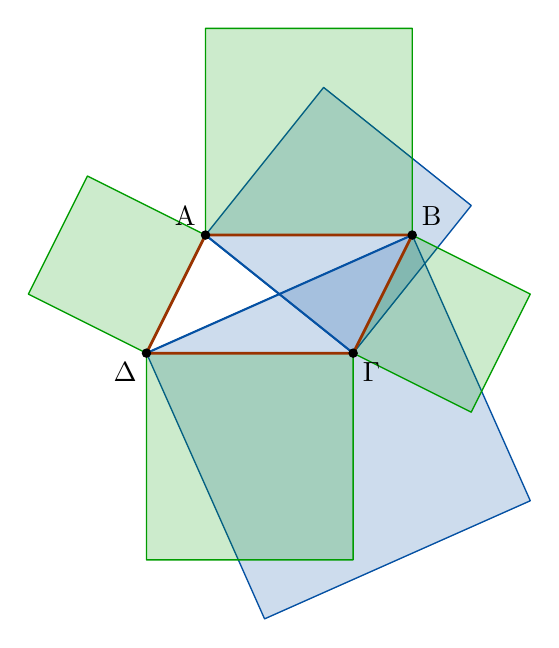
\begin{tikzpicture}[scale=.75]
\tkzSetUpLine[line width=1pt,color=black]
\tkzSetUpPoint[fill=black]

\tkzDefPoints{0/0/D,3.5/0/C,1/2/A,4.5/2/B}


\tkzDrawSegment[line width=0.75pt,color=BlueSqr](A,C)
\tkzDrawSegment[line width=0.75pt,color=BlueSqr](B,D)

\tkzDefSquare(A,C)
\tkzDrawPolygon[fill=BlueSqr,color=BlueSqr,fill opacity=0.2,line width=0.5pt](A,C,tkzFirstPointResult, tkzSecondPointResult)
\tkzDefSquare(B,D)
\tkzDrawPolygon[fill=BlueSqr,color=BlueSqr,fill opacity=0.2,line width=0.5pt](B,D,tkzFirstPointResult, tkzSecondPointResult)

\tkzDefSquare(A,B)
\tkzDrawPolygon[fill=RedSqr,color=RedSqr,fill opacity=0.2,line width=0.5pt](A,B,tkzFirstPointResult, tkzSecondPointResult)
\tkzDefSquare(B,C)
\tkzDrawPolygon[fill=RedSqr,color=RedSqr,fill opacity=0.2,line width=0.5pt](B,C,tkzFirstPointResult, tkzSecondPointResult)
\tkzDefSquare(C,D)
\tkzDrawPolygon[fill=RedSqr,color=RedSqr,fill opacity=0.2,line width=0.5pt](C,D,tkzFirstPointResult, tkzSecondPointResult)
\tkzDefSquare(D,A)
\tkzDrawPolygon[fill=RedSqr,color=RedSqr,fill opacity=0.2,line width=0.5pt](D,A,tkzFirstPointResult, tkzSecondPointResult)

\tkzDrawPolygon[color=ShapeClr](A,B,C,D)
\tkzDrawPoints[size=3](A,B,C,D)
\tkzLabelPoint[above left](A){$\rm A$}
\tkzLabelPoint[above right](B){$\rm B$}
\tkzLabelPoint[below right](C){$\rm \Gamma$};
\tkzLabelPoint[below left](D){$\rm \Delta$};

\end{tikzpicture}

\end{document}
